\section{Volume Inequalities}

\subsection{Spherical Sections of Symmetric Bodies}

Consider the $n$-dimensional cross-polytope $B_1^n$. The maximal ellipsoid in $B_1^n$ is the Euclidean ball of radius $1/\sqrt{n}$. If we take some orthogonal transformation $U$, then obviously, $U B_1^n$ contains the ball as well, and so does $B_1^n \cap U B_1^n$. But what if we instead consider the minimal ball that contains $B_1^n \cap U B_1^n$? We have the following remarkable theorem, which we prove later.

\begin{theorem}[Ka\u{s}in's Theorem]
\label{cross-polytope Kasin's theorem}
For each $n$, there is an orthogonal transformation $U$ such that $B_1^n\cap U B_1^n$ is contained in the (Euclidean) ball of radius $32/\sqrt{n}$.
\end{theorem}

The important thing to note here is the fact that just by intersecting just two copies of the cross-polytope, we manage to reduce the radius of the minimal circumscribing ball by a factor of $\sqrt{n}$! Indeed, this intersection is what we call ``approximately spherical" since its distance from the Euclidean ball is then at most $32$. The constant factor of $32$ can be improved upon as well.\\

For the same orthogonal transformation $U$, $\conv(Q\cup U Q)$ is at distance at most $32$ from the Euclidean ball as well (where $Q$ is $[-1,1]^n$).\\

How would one go about constructing such a transformation? The points of contact between the ball of radius $1/\sqrt{n}$ are those of the form $\left(\pm\frac{1}{n},\ldots,\pm\frac{1}{n}\right)$.\\
The points furthest away are those near the corners of the cross-polytope. So we would want to take a transformation whose facets ``chop off" these corners.\\

Recall that in the beginning, we had explained that the volume of the cross-polytope is $2^n/n!$, so if $r(\theta)$ is the radius of $B_1^n$ in the direction $\theta$, then

\begin{equation}
\label{eqn cross-polytope volume ratio limit}
    \int_{S^{n-1}} r(\theta)^n\d\sigma = \frac{2^n}{n! v_n} \leq \left(\frac{2}{\sqrt{n}}\right)^n.
\end{equation}

This feature wherein $r(\theta)$ is not expected to be much more than $2/\sqrt{n}$ is captured in the following definition.

\begin{fdef}[Volume Ratio]
Let $K$ be a convex body in $\R^n$. Then the \textit{volume ratio} of $K$ is defined as
\[ \vr(K) = \left(\frac{\vol(K)}{\vol(\mathcal{E})}\right)^{1/n} \]
where $\mathcal{E}$ is the maximal ellipsoid contained in $K$.
\end{fdef}

\Cref{eqn cross-polytope volume ratio limit} then says that $\vr(B_1^n)\leq 2$ for all $n$. Let us now prove (a slightly more general version of) Ka\u{s}in's Theorem, scaling everything up by $n$ for the sake of convenience.

\clearpage
\begin{ftheo}
\label{kasin's theorem orthogonal intersection}
Let $K$ be a symmetric convex body in $\R^n$ that contains $B_2^n$. Let
\[ R = \left(\frac{\vol(K)}{\vol(B_2^n)}\right)^{1/n}. \]
Then there is an orthogonal transformation $U$ of $\R^n$ such that
\[ K\cap U K \subseteq 8R^2 B_2^n. \]
\end{ftheo}

\begin{proof}
Denote by $\norm{\cdot}_K$ the norm under which $K$ is the unit ball. Observe that since $B_2^n\subseteq K$, $\norm{x}_K\leq \norm{x}$ for all $x\in\R^n$. Note that if $U$ is an orthogonal transformation, then the norm corresponding to $K\cap U K$ is the maximum of that corresponding to $K$ and $U K$ (at that point). Therefore, because the norm corresponding to $8R^2 B_2^n$ is $\frac{1}{8R^2}$ times the Euclidean norm, we just want to find an orthogonal transformation $U$ such that for all $\theta\in S^{n-1}$,
\[ \max(\norm{U\theta}_K, \norm{\theta}_K) \geq \frac{1}{8R^2}. \]
It suffices to show that for all $\theta\in S^{n-1}$,
\begin{equation}
\label{eqn kasin's theorem final aim}
    \frac{\norm{U\theta}_K + \norm{\theta}_K}{2} \geq \frac{1}{8R^2}.
\end{equation}
Now, note that the function $N$ given by $x\mapsto \frac{\norm{U x}_K + \norm{x}_K}{2}$ is a norm on $\R^n$. Also, it satisfies $N(x)\leq \norm{x}$ for all $x$.\\
We aim to show that $N$ is ``large" everywhere. Let $\phi$ be a point on the sphere such that $N(\phi) = t$. Then if $\norm{\theta-\phi} \leq t$, then
\[ N(\theta) \leq N(\phi) + N(\theta - \phi) \leq t + \norm{\theta-\phi} \leq 2t. \]
That is, for $\theta$ in a spherical cap of radius $t$ about $\phi$, $N(\theta)$ is at most $2t$. \Cref{spherical cap lower bound} implies that such a cap has measure  at least $\frac{1}{2}\left(\frac{t}{2}\right)^{n-1} \geq \left(\frac{t}{2}\right)^{n}$. Then, considering the integral over only the spherical cap, we have
\begin{equation}
\label{eqn kasin theorem integral lower bound}
    \int_{S^{n-1}} \frac{1}{N(\theta)^{2n}} \d\sigma \geq \frac{1}{(2t)^{2n}}\left(\frac{t}{2}\right)^n = \frac{1}{2^{3n}t^n}.
\end{equation}

Now, we claim that there is an orthogonal transformation $U$ such that
\begin{equation}
\label{eqn kasin theorem integral upper bound}
    \int_{S^{n-1}} \frac{1}{N(\theta)^{2n}}\d\sigma \leq R^{2n}.
\end{equation}

Because $N(\theta)^2 \geq \norm{\theta}_K \norm{U\theta}_K $, it suffices to show the existence of an orthogonal transformation $U$ such that
\[ \int_{S^{n-1}} \frac{1}{\norm{\theta}^n_K\norm{U\theta}^n_K}\d\sigma \leq R^{2n}. \]

We prove this probabilistically. Consider the average over all orthogonal transformations $U$ of some function $f$ on the sphere. This should just be the average of the value of $f$ over the entire sphere. That is,
\[ \avg_U f(U \theta) = \int_{S^{n-1}} f(\phi) \d\sigma(\phi). \]
Setting $f$ as the function given by
\[ \theta \mapsto \frac{1}{\norm{\theta}_K^n}, \]
we have the following:
\begin{align*}
    \avg_U \left(\int_{S^{n-1}} \frac{1}{\norm{U\theta}^n_K\norm{\theta}^n_K} \d\sigma(\theta) \right) &= \int_{S^{n-1}} \left( \avg_U\frac{1}{\norm{U\theta}^n_K} \right)\frac{1}{\norm{\theta}^n_K}\d\sigma(\theta) \\
    &= \int_{S^{n-1}} \left( \int_{S^{n-1}} \frac{1}{\norm{\phi}^n_K} \d\sigma(\phi) \right)\frac{1}{\norm{\theta}^n_K}\d\sigma(\theta) \\
    &= \left(\int_{S^{n-1}}\frac{1}{\norm{\theta}^n_K}\d\sigma(\theta)\right)^2 = R^{2n},
\end{align*}
where the last equality follows from \Cref{eqn volume in terms of body's norm}. Since the average of the integral over orthogonal transformations is at most $R^{2n}$, there must be some orthogonal transformation $U$ such that the integral is at most $R^{2n}$ and \Cref{eqn kasin theorem integral upper bound} holds! Then, combining \Cref{eqn kasin theorem integral lower bound} and \Cref{eqn kasin theorem integral upper bound}, we get
\[ \frac{1}{2^{3n}t^n} \leq R^{2n} \implies t \geq \frac{1}{8R^2}. \]
That is, for any $\phi\in S^{n-1}$, $\norm{\phi}_K \geq \frac{1}{8R^2}$, which is exactly what we set out to show in \Cref{eqn kasin's theorem final aim}!
\end{proof}

Due to the probabilistic nature of the above proof, we do not actually get an orthogonal transformation $U$. However, a question that might come to mind is - do there exist symmetric bodies for which we \textit{can} explicitly construct $U$?\\
Consider the simple case of the cross-polytope. As mentioned towards the beginning of this section, we would like to ``chop off" the corners. A relatively obvious method to do this that comes to mind is to construct a transformation such that the direction of each of the new corners coincides with the directions of the centers of the original facets. In $2$ dimensions, such an orthogonal transformation just means we rotate $B_1^2$ by $45^\circ$.\\

However, does such an orthogonal transformation exist for the cross-polytope in any general dimension? Stating it more rigorously, we want to determine for each $n$ if there is an orthogonal transformation $U$ such that for each standard basis vector $e_i$ of $\R^n$, $U e_i$ is $\sqrt{n}$ times one of the vectors of the form $(\pm \frac{1}{n},\ldots,\pm \frac{1}{n})$.\\
That is, we are looking for an $n\times n$ orthogonal matrix with each entry as $\pm \frac{1}{\sqrt{n}}$. Such a matrix without the $\sqrt{n}$ factor (it then merely requires that the rows are orthogonal) is known as a \textit{Hadamard matrix}. For $n\leq 2$, there obviously exist Hadamard matrices
\[
\begin{pmatrix}
1
\end{pmatrix}
\text{ and }
\begin{pmatrix}
+1 & +1 \\
+1 & -1
\end{pmatrix}.
\]
It may be shown that if a Hadamard matrix of dimension $n>2$ exists, then $n$ is a multiple of $4$.\footnote{Let $H$ be a Hadamard matrix. We may assume that all the elements in the first row are $+1$. Let $a$, $b$, $c$ and $d$ be the number of columns starting with $(+,+,+)$, $(+,+,-)$, $(+,-,+)$ and $(+,-,-)$ respectively. We trivially have $a+b+c+d=n$. Using the pairwise orthogonality of the first $3$ rows, we get $3$ other conditions which enable us to conclude that $n=4a$.} However, it is unknown which multiples of $4$ Hadamard matrices do indeed exist for. It is known that they do exist for $n$ a power of $2$, but even these (known as \textit{Walsh matrices}) don't give good estimates. There are good reasons\footnote{see Ramsey Theory.} for believing that we cannot explicitly find an orthogonal transformation that would give the right estimates.\\

Now, with the aid of \Cref{kasin's theorem orthogonal intersection}, proving \Cref{cross-polytope Kasin's theorem} is near-straightforward.\\
Recall how in the beginning of this section, we had stated that for the same orthogonal transformation $U$ that is mentioned in \Cref{kasin's theorem orthogonal intersection}, $\conv(Q\cup U Q)$ is at distance $32$ from the Euclidean ball, where $Q=[-1,1]^n$. However, we cannot get an approximately spherical body by taking the intersection as we have in \Cref{kasin's theorem orthogonal intersection}.\\
Dually, we cannot get an approximately spherical body by taking the convex hull of a union for a cross-polytope. Both of these ideas (of taking the convex hull \textit{and} the intersection) are combined in the following fascinating result of Milman's.

\begin{ftheo}[QS-Theorem]
There is a constant $M$ such that for all symmetric convex bodies $K$ (of any dimension), there are linear maps $Q$ and $S$ and an ellipsoid $\mathcal{E}$ such that if $\tilde K = \conv(K\cup Q K)$, then
\[ \mathcal{E} \subseteq \tilde K \cap S \tilde K \subseteq M\mathcal{E}. \]
\end{ftheo}

Note that $M$ is a universal constant independent of \textit{everything}. Here the ``QS" means ``quotient of a subspace".

\clearpage
\subsection{The Pr\'{e}kopa-Leindler Inequality}

\subsubsection{Brunn's Theorem}

Consider some convex body $K$ in $\R^2$ and the map $v:\R\to\R$ such that $r$ maps to the length (the Lebesgue measure in $\R$) of the intersection of the line $x=r$ with the body $K$. We can think of this as ``collapsing" the body onto the $x$-axis like a deck of cards. To understand this better, consider the following image which represents the graph of $v$ for $K$.\footnote{Source: An Introduction to Modern Convex Geometry by Keith Ball.}

\begin{center}
    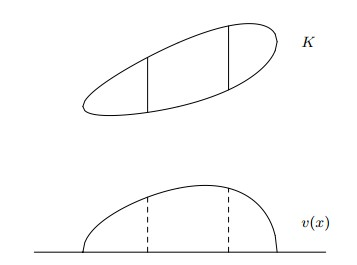
\includegraphics{brunn-shakedown.jpg}
\end{center}

It may be shown that for any convex body $K$ in $\R^2$, the corresponding function $v$ is concave on its support.\\

How would one go about generalizing this $v$ to a higher dimensional $K$, say in $3$ dimensions? As might be expected, the function $v:\R\to\R$ maps $r$ to the Lebesgue measure (in $\R^2$) of the intersection of $x=r$ with the body $K$.\\
Does this $v$ need to be concave? No, it does not! Consider a cone - say the one given by
\[\{(x,y,z)\in\R^3 : y^2+z^2\leq x^2, x\geq 0\}.\]
Then since the area of the intersection grows as $x^2$, the function is quite obviously not concave. However, the cone is a ``maximal" convex body in some sense, it is just barely convex and the curved surface is composed of lines. One might now note that the function $r\mapsto \sqrt{v(r)}$ for the cone is indeed (barely) concave! Brunn perhaps noticed this pattern and proved an analogous result for higher dimensions.

\begin{ftheo}[Brunn's Theorem]
\label{brunn's theorem}
Let $K$ be a convex body in $\R^n$, $u$ a unit vector in $\R^n$, and for each $r$, define
\[ H_r = \{x\in\R^n : \langle x,u\rangle = r\}. \]
Then, the function
\[ v:r\mapsto \vol(H_r\cap K)^{1/(n-1)} \]
is concave on its support.
\end{ftheo}

A consequence of this theorem is that given any centrally symmetric body in $\R^n$, the $(n-1)$-dimensional slice with the largest area orthogonal to some fixed unit vector $u$ is that through the origin!

\subsubsection{The Brunn-Minkowski Inequality}

Brunn's Theorem was turned from an idle observation to an extremely powerful tool by Minkowski in the form of the Brunn-Minkowski inequality. We omit the proof of Brunn's Theorem as it is obvious from this inequality, which we state shortly.\\

Before we do this, let us introduce some notation. If $X$ and $Y$ are sets in $\R^n$ and $\alpha,\beta\in\R$, then we write
\[ \alpha X + \beta Y = \{ \alpha x + \beta y : x \in X, y \in Y \}. \]
This method of using addition in $\R^n$ to define the addition of sets in $\R^n$ is known as \textit{Minkowski addition}.\\
In the context of Brunn's Theorem, consider three parallel slices $A_r$,$A_s$, and $A_t$ of a body $K$ in $\R^n$ at positions $r$, $s$, and $t$. These slices can be thought of as subsets of $\R^{n-1}$. Further suppose that $r<s<t$ and we have $\lambda\in(0,1)$ such that $s = \lambda r + (1-\lambda)t$. Note that due to the convexity of $K$, 
\[A_s \supseteq \lambda A_r + (1-\lambda)A_t.\]
All Brunn's Theorem says is that
\[ \vol(A_s)^{1/(n-1)} \geq \lambda \vol(A_r)^{1/(n-1)} + (1-\lambda) \vol(A_t)^{1/(n-1)}. \]
Observe that we have removed any remnant of $\R^n$ from this equation. Cleaning it up and restating it more generally, we have the following.

\begin{ftheo}[Brunn-Minkowski Inequality]
\label{brunn minkowski inequality}
Let $A$ and $B$ be two non-empty compact subsets of $\R^n$. Then for any $\lambda\in[0,1]$,
\begin{equation}
\label{eqn brunn minkowski inequality}
    \vol(\lambda A + (1-\lambda) B)^{1/n} \geq \lambda\vol(A)^{1/n} + (1-\lambda)\vol(B)^{1/n}.
\end{equation}
\end{ftheo}
It is quite obvious that given the above inequality, Brunn's Theorem is true. Here, the non-emptiness of $A$ and $B$ correspond to the fact that we restrict $v$ to the support in Brunn's Theorem.\\

We encourage the reader to show that \Cref{eqn brunn minkowski inequality} is equivalent to
\begin{equation}
\label{eqn brunn minkowski inequality alt no lambda}
    \vol(A+B)^{1/n} \geq \vol(A)^{1/n} + \vol(B)^{1/n}
\end{equation}

We omit the proof of the Brunn-Minkowski inequality and instead show how it follows from the far more powerful, near-magical Pr\'{e}kopa-Leindler inequality.\\
Before we do this, let us show how the popular isoperimetric inequality follows from the Brunn-Minkowski inequality.

\begin{theorem}[Isoperimetric Inequality]
\label{isoperimetric inequality}
Among bodies of a given volume, Euclidean balls have the least surface area.
\end{theorem}
\begin{proof}
Let $C$ be a compact body of volume equal to that of $B_2^n$. The ($(n-1)$-dimensional) ``surface area" of $C$ is equal to
\[ \vol(\partial C) = \lim_{\varepsilon\to 0} \frac{\vol(C + \varepsilon B_2^n) - \vol(C)}{\varepsilon}. \]
\Cref{eqn brunn minkowski inequality alt no lambda} implies that
\begin{align*}
    \vol(C+\varepsilon B_2^n) &\geq \left(\vol(C)^{1/n} + \varepsilon\vol(B_2^n)^{1/n}\right)^{n} \\
    &\geq \vol(C) + n\varepsilon\vol(B_2^n)^{1/n}\vol(C)^{(n-1)/n}.
\end{align*}
Then,
\begin{align*}
    \vol(\partial C) &\geq \lim_{\varepsilon\to 0} \frac{n\varepsilon\vol(B_2^n)^{1/n}\vol(C)^{(n-1)/n}}{\varepsilon}\\
    &= n\vol(B_2^n) = \vol(\partial B_2^n).\qedhere
\end{align*}
\end{proof}

It may also be shown using the \nameref{brunn minkowski inequality} and the weighted AM-GM inequality that for any compact subsets $A,B$ of $\R^n$,
\begin{equation}
\label{eqn multiplicative brunn minkowski}
    \vol(\lambda A + (1-\lambda)B) \geq \vol(A)^{\lambda} \vol(B)^{1-\lambda}
\end{equation}
The above equation is more commonly known as the \textit{multiplicative Brunn-Minkowski inequality}, while \Cref{eqn brunn minkowski inequality} is known as the \textit{additive Brunn-Minkowski inequality}. It may also be shown that while this is weaker than the Brunn-Minkowski inequality for \textit{particular} subsets $A$ and $B$, the two are equivalent if we know \Cref{eqn multiplicative brunn minkowski} for \textit{all} $A$ and $B$.

\begin{proof}[Multiplicative Brunn-Minkowski implies additive Brunn-Minkowski]
Fix some $\lambda\in[0,1]$ and let
\[ \lambda' = \dfrac{\dfrac{\lambda}{\vol(B)^{1/n}}}{\dfrac{\lambda}{\vol(B)^{1/n}} + \dfrac{1-\lambda}{\vol(A)^{1/n}}}. \]
Applying \Cref{eqn multiplicative brunn minkowski}, we get
\[ \vol\left(\lambda'\frac{A}{\vol(A)^{1/n}} + (1-\lambda')\frac{B}{\vol(B)^{1/n}}\right) \geq 1. \]
Also,
\[
    \lambda'\frac{A}{\vol(A)^{1/n}} + (1-\lambda')\frac{B}{\vol(B)^{1/n}} =  \frac{\lambda A + (1-\lambda)B}{\lambda\vol(A)^{1/n} + (1-\lambda)\vol(B)^{1/n}}.
\]
Therefore,
\[ \vol(\lambda A + (1-\lambda)B) \geq \left(\lambda\vol(A)^{1/n} + (1-\lambda)\vol(B)^{1/n}\right)^n, \]
which is just additive Brunn-Minkowski.
\end{proof}

This form is slightly more advantageous because there is no mention of the dimension $n$ or the non-emptiness of $A$ and $B$.

\subsubsection{The Pr\'{e}kopa-Leindler inequality}

The Pr\'{e}kopa-Leindler inequality that we mentioned earlier is essentially a generalization of the Brunn-Minkowski inequality to a more functional form, similar to how the Cauchy-Bunyakovasky-Schwarz inequality is a functional analogue of the Cauchy-Schwarz inequality.\\

To get a little more intuition for how the Brunn-Minkowski inequality is connected to the Pr\'{e}kopa-Leindler inequality, define $f$ as the indicator function on $A$, $g$ as the indicator function on $B$, and $m$ as the indicator function on $\lambda A+(1-\lambda)B$, .\footnote{the indicator function on $X$ for $X\subseteq \R^n$ is the map from $\R^n$ to $\{0,1\}$ such that $f(x)=1$ if $x\in X$ and $0$ otherwise.} Then \Cref{eqn multiplicative brunn minkowski} says
\[ \int_{\R^n} m \geq \left(\int_{\R^n}f\right)^\lambda \left(\int_{\R^n}g\right)^{1-\lambda}. \]
What is the relation between $m$, $f$, and $g$ that perhaps leads to this inequality being true? If for some $x$ and $y$, $f(x)=1$ and $g(y)=1$, then we have $m(\lambda x + (1-\lambda)y)=1$ as well. Therefore, for any $x,y\in\R^n$
\[ m(\lambda x + (1-\lambda)y) \geq f(x)^{\lambda}g(y)^{1-\lambda}. \]
It turns out that this condition is enough to conclude \Cref{eqn multiplicative brunn minkowski}!

\begin{ftheo}[Pr\'{e}kopa-Leindler inequality]
\label{prekopa leindler}
Let $f$, $g$ and $m$ be non-negative measurable functions on $\R^n$ and $\lambda\in(0,1)$ such that for all $x,y\in\R^n$,
\begin{equation}
\label{eqn prekopa leindler}
    m(\lambda x + (1-\lambda)y) \geq f(x)^{\lambda}g(y)^{1-\lambda}.
\end{equation}
Then,
\[ \int_{\R^n} m \geq \left(\int_{\R^n}f\right)^\lambda \left(\int_{\R^n}g\right)^{1-\lambda}. \]
\end{ftheo}

The astute reader might notice that this is something of a reversed H\"{o}lder's inequality, which says that if we have non-negative functions $f$ and $g$ and define $m$ by $m(z) = f(z)^{\lambda}g(z)^{1-\lambda}$ for each $z$, then
\begin{equation}
\label{eqn holder's inequality}
    \int m \leq \left(\int f\right)^\lambda \left(\int g\right)^{1-\lambda}.
\end{equation}

The difference is that in the Pr\'{e}kopa-Leindler inequality, we have
\[ m(\lambda x + (1-\lambda)y) \geq \sup_{x,y} f(x)^\lambda g(x)^{1-\lambda}, \]
whereas in H\"older's, we only consider the pair $(x,y)=(z,z)$.\\

\begin{proof}[Proof of one-dimensional Brunn-Minkowski inequality]
Suppose $A$ and $B$ are non-empty measurable subsets of $\R$. We use $\norm{\cdot}$ to represent the Lebesgue measure on $\R$.\\
We can assume that $A$ and $B$ are compact\footnote{due to the \href{https://en.wikipedia.org/wiki/Regular_measure}{inner regularity} of the Lebesgue measure.}. We can now shift both sets and assume that $A\cap B = \{0\}$. However, in this case, we have $A\cup B\subseteq A+B$ and so, due to the almost-disjointedness of $A$ and $B$,
\[ \norm{A+B} \geq \norm{A\cup B} = \norm{A}+\norm{B}. \]
This is just \Cref{eqn brunn minkowski inequality alt no lambda}.
\end{proof}

\begin{proof}[Proof of one-dimensional Pr\'{e}kopa-Leindler inequality]
We have non-negative measurable functions $f$, $g$, and $m$. We use $\norm{\cdot}$ to represent the Lebesgue measure on $\R$. For any function $h:\R\to\R$ and $t\in\R$, define
\[ L_h(t) = \{x\in\R: h(x)\geq t\}. \]
Then note that by \Cref{eqn prekopa leindler},
\[ L_m(t) \supseteq \lambda L_f(t) + (1-\lambda)L_g(t). \]
We can then apply the one-dimensional Brunn-Minkowski inequality to get
\[ \norm{L_m(t)} \geq \norm{\lambda L_f(t) + (1-\lambda)L_g(t)} \geq \lambda \norm{L_f(t)} + (1-\lambda)\norm{L_g(t)}. \]
Finally, we can assume boundedness of all three functions and use Fubini's Theorem to say that
\begin{align*}
    \int m  &= \int \norm{L_m(t)}\d t \\
    &\geq \lambda \int \norm{L_f(t)}\d t + (1-\lambda) \int \norm{L_g(t)}\d t \\
    &= \lambda \int f + (1-\lambda) \int g \\
    &\geq \left(\int f\right)^{\lambda}\left(\int g\right)^{1-\lambda},
\end{align*}
where the last step follows from the weighted AM-GM inequality.
\end{proof}

\begin{proof}[Proof of Pr\'{e}kopa-Leindler inequality]
We prove this inductively. Suppose we have $m$, $f$, and $g$ from $\R^n\to\R$ ($n>1$) satisfying \Cref{eqn prekopa leindler}. For any $z\in\R$ and any function $h:\R^n\to \R$, we denote by $h_z:\R^{n-1}\to\R$ the function given by $h_z(x)=h(x,z)$ (for $z\in\R^{n-1}$) -- we make the last coordinate constant and consider the resulting function on the remaining $n-1$ coordinates. Now, let $\alpha,\beta\in\R$, $x,y\in\R^{n-1}$ and let $\gamma = \lambda\alpha + (1-\lambda)\beta$. Then,
\begin{align*}
    m_\gamma(\lambda x + (1-\lambda)y) &= m(\lambda x + (1-\lambda)y, \lambda\alpha + (1-\lambda)\beta) \\
    &\geq f(x,\alpha)^\lambda g(y,\beta)^{1-\lambda} \\
    &= f_\alpha(x)^\lambda g_\beta(y)^{1-\lambda}.
\end{align*}
That is, $m_\gamma$, $f_\alpha$, and $g_\beta$ satisfy \Cref{eqn prekopa leindler} (on $\R^{n-1}$). We can then apply the inductive hypothesis on them to get
\[ \int_{\R^{n-1}} m_\gamma \geq \left(\int_{\R^{n-1}}f_\alpha\right)^\lambda \left(\int_{\R^{n-1}}g_\beta\right)^{1-\lambda}. \]
Now, for any function $h:\R^n\to\R$, we denote by $\tilde{h}:\R\to\R$ the function given by
\[ \gamma \mapsto \int_{\R^{n-1}} f_\gamma. \]
Note that the functions $\tilde{m}$, $\tilde{f}$, and $\tilde{g}$ satisfy the condition for the one-dimensional Pr\'{e}kopa-Leindler inequality! Therefore, condensing the iterated integral to a joint integral, we get
\[ \int_{\R^n} m \geq \left(\int_{\R^n} f\right)^{\lambda}\left(\int_{\R^n} g\right)^{1-\lambda}, \]
which is exactly what we desire!
\end{proof}

This proof is quite magical - we use the inequality on $\R^{n-1}$ and $\R^1$ with barely any extra work to conclude that it holds for $\R^n$.

To conclude this section, we state another surprising result (from \cite{Busemann1949}) in a similar vein to the nice observation that is Brunn's Theorem.

\begin{theorem}[Busemann's Theorem]
Let $K$ be a symmetric convex body in $\R^n$ and for each unit vector $u$, let $r(u)$ be the volume of the slice of $K$ by the subspace orthogonal to $u$. Then the body whose radius in each direction $u$ is $r(u)$ is convex as well.
\end{theorem}

\subsection{The Reverse Isoperimetric Problem}
\label{subsection: reverse isoperimetric problem 2.3}

The \nameref{isoperimetric inequality} solves the problem of finding the body with the largest volume among bodies with a given surface area. How would one go about solving the reversed problem -- finding the body with the largest surface area among bodies with a given volume? We must phrase this more carefully such that it makes sense because as it stands, we could make the surface area arbitrarily large (consider a large thin disc). So the more common way of phrasing it is -- given a convex body, how small can we make its surface area by applying an affine transformation that preserves volume?

\begin{theorem}
\label{reverse isoperimetric}
Let $K$ be a convex body, $T$ a regular solid simplex in $\R^n$, and $Q$ a cube in $\R^n$. Then, there is an affine transformation $\tilde{K}$ of $K$ such that the volume of $\tilde{K}$ is equal to that of $T$ and whose surface area is at most that of $T$. If $K$ is symmetric, then there is an affine transformation $\tilde{K}$ of $K$ such that the volume of $\tilde{K}$ is equal to that of $Q$ and whose surface area is at most that of $Q$.
\end{theorem}

The primary focus of this section is to find the bodies with the largest volume ratios -- this is answered for symmetric bodies in \Cref{symmetric volume ratio cube}, which we encourage the reader to look at now.\\

Given this, we can prove the second part of \Cref{reverse isoperimetric} as follows.

Choose $\tilde{K}$ such that its maximal ellipsoid is $B_2^n$. Then $\tilde{K}$ has volume at most $2^n$ (since this is the volume of the cube with maximal ellipsoid $B_2^n$). Note that
\[ \vol(\partial Q) = 2n\vol(Q)^{(n-1)/n}. \]
Therefore, we shall show that
\[ \vol(\partial \tilde{K}) \leq 2n\vol(\tilde{K})^{(n-1)/n} \]
Indeed, we have
\begin{align*}
    \vol(\partial \tilde K) &= \lim_{\varepsilon\to 0}\frac{\vol(\tilde{K}+\varepsilon B_2^n) - \vol(\tilde{K})}{\varepsilon} \\
    &\leq \lim_{\varepsilon\to 0} \frac{\vol(\tilde{K}+\varepsilon \tilde{K}) - \vol(\tilde{K})}{\varepsilon} & (\text{because }B_2^n\subseteq \tilde{K}) \\
    &= \vol(\tilde{K}) \lim_{\varepsilon\to 0} \frac{(1+\varepsilon)^n - 1}{\varepsilon} \\
    &= n \vol(\tilde K) \\
    &= n \vol(\tilde{K})^{1/n} \vol(\tilde{K})^{(n-1)/n} \\
    &\leq 2n \vol(\tilde{K})^{(n-1)/n}. & (\text{by \Cref{symmetric volume ratio cube}})
\end{align*}

\subsubsection{Volume Ratio Estimates and Young's Convolution Inequality}

\begin{ftheo}
\label{symmetric volume ratio cube}
Among symmetric convex bodies, the cube has the largest volume ratio.
\end{ftheo}

The above is equivalent to saying that if $K$ is a convex body whose maximal ellipsoid is $B_2^n$, then $\vol(K)\leq 2^n$. By \nameref{fritz john's theorem}, there exist unit vectors $(u_i)$ and positive $(c_i)$,
\[ \sum_i c_i u_i\otimes u_i = I_n. \]
Consider the polytope
\begin{equation}
\label{eqn symmetric volume ratio cube polytope}
    C = \{ x\in\R^n : |\langle x,u_i\rangle| \leq 1\text{ for }1\leq i\leq m\}.    
\end{equation}

We clearly have $K\subseteq C$, so it suffices to show that $\vol(C) \leq 2^n$.\\
The most important tool we use for this is the following.

\begin{theorem}[Young's Convolution Inequality]
\label{young's convolution inequality}
Suppose $f\in L^p(\R)$, $g\in L^q(\R)$, and $\frac{1}{p} + \frac{1}{q} = 1 + \frac{1}{s}$. Then,
\begin{equation}
\label{eqn young's convolution inequality}
    \norm{f * g}_s \leq \norm{f}_p \norm{g}_q,
\end{equation}
\end{theorem}

In the above, $f * g$ represents the \textit{convolution} of $f$ and $g$ and is the function given by
\[ x \mapsto \int_{\R} f(x) g(x-y) \d{y}. \]

In compact spaces, equality holds in \Cref{eqn young's convolution inequality} when $f$ and $g$ are constant functions.\\
On $\R$ however, we can add a multiplicative constant $c_{p,q}<1$ on the right and improve the inequality. Here, equality holds when $f$ and $g$ are appropriate Gaussians $x\mapsto e^{-a x^2}$ and $x\mapsto e^{-b x^2}$, where $a$ and $b$ are some constants depending on $p$ and $q$.\footnote{see \href{https://www.sciencedirect.com/science/article/pii/0001870876901845}{this paper} by Brascamp and Lieb.} \\
Young's inequality is often written in an alternate form. Let $r$ be equal to $1-\frac{1}{s}$. We then have $\frac{1}{p} + \frac{1}{q} + \frac{1}{r} = 2$. Let $h$ be a function such that $\norm{h}_r=1$ and
\[ \norm{(f*g)(h)}_1 = \norm{f*g}_s \norm{h}_r. \]
We know that such a $h$ exists by choosing that which satisfies the equality condition in H\"older's inequality.

Therefore, rewriting the above in terms of $h$,

\[ \norm{(f*g)(h)} \leq \norm{f}_p \norm{g}_q \norm{h}_r. \]

More explicitly,

\[ \int \int f(y) g(x-y) h(x) \d{y} \d{x} \leq \norm{f}_p \norm{g}_q \norm{h}_r. \]

Equivalently,

\[ \int \int f(y) g(x-y) h(-x) \d{y} \d{x} \leq \norm{f}_p \norm{g}_q \norm{h}_r. \]

Note that $(y) + (x-y) + (-x) = 0$. Consider the map from $\R^2\to \R^3$ given by
\[ (x,y) \mapsto (y,x-y,-x). \]
The image of this transformation is equal to
\[ H = \{(u,v,w):u+v+w=0\}. \]
Therefore, if $\frac{1}{p} + \frac{1}{q} + \frac{1}{r} = 2$,
\[ \int_H f(u)g(v)h(w) \leq \norm{f}_p \norm{g}_q \norm{h}_r. \]
We integrate over a two-dimensional measure on the subspace $H$.\\

\subsubsection{A Generalization}

So this is all well and good, but how is it related to volume ratios? The paper of Brascamp and Lieb mentioned in a footnote previously did more than just say that equality holds when the functions are appropriate Gaussians. It actually \textit{generalized} Young's Convolution Inequality to higher-dimensional spaces and any number of functions. Note that the map from $\R^2$ to $\R^3$ that leads to $H$ is given by
\[ x \mapsto (\langle x,v_1\rangle, \langle x,v_2\rangle, \langle x,v_3\rangle), \]
where $v_1 = (0,1)$, $v_2 = (1,-1)$, and $v_3 = (-1,0)$. The generalisation led to the following:
\begin{theorem}
If $(v_i)_1^m$ are vectors in $\R^n$ and $(p_i)_1^m$ are positive numbers satisfying
\[ \sum_i \frac{1}{p_i} = n \]
and $(f_i)_1^m$ are non-negative measurable functions on $\R$, then the expression
\[ \dfrac{\displaystyle\int_{\R^n} \displaystyle\prod_{i=1}^m f_i(\langle x,v_i\rangle) }{\displaystyle\prod_{i=1}^m \norm{f_i}_{p_i}} \]
is ``maximized"\footnote{there are degenerate cases for which the maximum is not attained} when the $(f_i)$ are appropriate Gaussian densities $f_i(x) = e^{-\alpha_i x^2}$, where each $\alpha_i$ depends on the $(p_i)$, $(v_i)$, $m$, and $n$.
\end{theorem}

However, this seems quite unwieldy. The constants $\alpha_i$ are quite difficult to compute since they result from non-linear equations of all the variables. When we talk about convex bodies however, this issue completely disappears and gives a surprising connection back to \nameref{fritz john's theorem}!

\begin{ftheo}
\label{ball volume ratio estimate prereq}
If $(u_i)_1^m$ are unit vectors in $\R^n$, $(c_i)_1^m$ are positive reals, and $(f_i)_1^m$ are non-negative measurable functions such that
\[ \sum_{i=1}^m c_i u_i\otimes u_i = I_n, \]
and
\[ \int_{\R^n} \prod_{i=1}^m f_i(\langle x,u_i\rangle)^{c_i} \leq \prod_{i=1}^m \left(\int f_i\right)^{c_i} \]
\end{ftheo}

A couple of things to note here are:
\begin{itemize}
    \item The maximized value is $1$ now! The inequality is sharp.
    \item The $c_i$ play the role of the $\frac{1}{p_i}$. As observed earlier, the $(c_i)$ sum up to $1$ just like the $(\frac{1}{p_i})$ should.
    \item We replace each $f_i$ with $f_i^{c_i}$ to make it easier to state the equality condition.
\end{itemize}

When each $f_i$ is equal to $t\mapsto e^{-t^2}$,
\begin{align*}
    \int_{\R^n} \prod_{i=1}^m f_i(\langle x,u_i\rangle)^{c_i} &= \int_{\R^n} \exp\left(-\sum_i c_i \langle x,u_i\rangle^2\right) \\
    &= \int_{\R^n} \exp(-\norm{x}^2) \\
    &= \int_{\R^n} \exp\left(-\sum_i x_i^2\right) \\
    &= \left(\int e^{-t^2}\right)^n \\
    &= \left(\int e^{-t^2}\right)^{\sum_i c_i} \\
    &= \prod_{i=1}^m \left(\int f_i\right)^{c_i}
\end{align*}

We now prove \Cref{symmetric volume ratio cube}.

\begin{proof}
Let $K$ be a convex body with maximal ellipsoid $B_2^n$, $(u_i)_1^m$ and $(c_i)_1^m$ be the points and constants as mentioned in \nameref{fritz john's theorem}, and $C$ be the polytope defined in \Cref{eqn symmetric volume ratio cube polytope}. For each $1\leq i\leq m$, define $f_i:\R\to\R$ to be the indicator function on $[-1,1]$. Observe that for $x\in\R^n$, $f_i(\langle x,u_i\rangle)$ is non-zero for every $i$ if and only if $|\langle x,u_i\rangle|\leq 1$ for every $i$, that is, $x\in C$. Therefore,
\begin{align*}
    \vol(C) &= \int_{\R^n} \prod_{i=1}^m f_i(\langle x,u_i\rangle)^{c_i} \\
    &\leq \prod_{i=1}^m \left(\int f_i\right)^{c_i} \\
    &= \prod_{i=1}^m 2^{c_i} = 2^n,
\end{align*}
which proves our claim.
\end{proof}

The analogous result of \Cref{symmetric volume ratio cube} for general convex bodies, as might be expected, says that among convex bodies, the regular solid simplex has the largest volume ratio.